% ===========================================================================
% The Compilable Frontier as a Characterization Theorem
% ===========================================================================
\subsection{The Compilable Frontier: A Characterization Theorem}
\label{sec:characterization}

Theorem~\ref{thm:svnn_conditions} established that SVNN Conditions~1--2 are
\textit{sufficient} for design-time certification. Theorem~\ref{thm:necessity}
(NP-hardness) established that violating Condition~1 makes \textit{tight}
bound computation intractable. Here we close the gap: we prove that within
the class of affine abstract interpretations, Conditions~1--2 are
\textit{necessary} for dimension-optimal certification---the bound per layer
scales as $O(d \cdot r^2)$ for SVNN architectures but degrades to
$\Omega(d^2 \cdot r^2)$ for architectures violating Condition~1.

\vspace{4pt}
\begin{kingthm}[Compilable Frontier Characterization]
\label{thm:characterization}
Let $\mathcal{N}$ be a feedforward neural network with $L$ layers, maximum
width $d$, and $C^2$ activation functions on compact domain $X \subset
\mathbb{R}^{d_{\text{in}}}$. Consider any sound affine abstract
interpretation $\mathcal{A}$ (including DA, IA, and zonotope domains)
that propagates error bounds of the polynomial form
$B^{(\ell)} = J^{(\ell)} \cdot r + H^{(\ell)} \cdot r^2 + O(r^3)$
through each layer. Then:

\begin{enumerate}[label=(\roman*)]
    \item \textbf{Sufficiency (Theorem~\ref{thm:svnn_conditions}):}
    If $\mathcal{N}$ satisfies Conditions~1--2, then
    $B_{\text{total}} = O(L \cdot d \cdot r^2)$---the
    \textit{dimension-optimal} scaling for any affine method.

    \item \textbf{Necessity (new):}
    If $\mathcal{N}$ violates Condition~1 (coupled linear+nonlinear ops),
    then the error amplification factor per layer is
    $\|W^{(\ell)}\|_{1,\infty} = \Theta(\sqrt{d})$ under standard
    initialization, compared to the $d$-independent contractivity
    constant $\gamma < 1$ for SVNN architectures satisfying
    Condition~3. Multi-layer propagation yields
    $B_{\text{total}} = \Theta(d^{L/2} \cdot r^2)$ for non-SVNN vs.
    $B_{\text{total}} = O(L \cdot d \cdot r^2)$ for SVNN---an
    exponential-in-depth gap.
\end{enumerate}

Condition~1 is thus \textbf{necessary and sufficient} for
dimension-optimal affine certification of neural networks.
\label{thm:frontier}
\end{kingthm}

\vspace{2pt}
\noindent\textit{Proof of Necessity (Sharp Lower Bound).}
We construct a deterministic adversarial MLP achieving the theoretical
lower bound exactly.

\vspace{2pt}
\noindent\textbf{Step 1 (Adversarial MLP construction).}
Consider an MLP layer with weight matrix $W = \frac{1}{\sqrt{d}} \cdot J_d$,
where $J_d \in \mathbb{R}^{d \times d}$ is the all-ones matrix. The
$\ell_{1,\infty}$ norm is:
\begin{equation}
\|W\|_{1,\infty} = \max_{j} \sum_{i=1}^{d} |W_{j,i}|
= d \cdot \frac{1}{\sqrt{d}} = \sqrt{d}
\label{eq:sharp_l1inf}
\end{equation}

This is a \textbf{sharp} bound: no weight matrix with the same
Frobenius-norm budget ($\|W\|_F = 1$) can achieve a larger
$\ell_{1,\infty}$ norm ($\|W\|_{1,\infty} \leq \sqrt{d}\|W\|_F$,
tight exactly when all entries have equal magnitude). With ReLU
activation ($L_\sigma = 1$) and the adversarial weight matrix,
the per-layer error amplification is:
\begin{equation}
\|W \cdot (\mathbf{x} + \boldsymbol{\delta}) - W \cdot \mathbf{x}\|_\infty
\leq \sqrt{d} \cdot \|\boldsymbol{\delta}\|_\infty
\label{eq:sharp_amplification}
\end{equation}

The all-ones construction \textit{achieves} this bound with equality:
for $\mathbf{x} = [1,\ldots,1]^T$ and $\boldsymbol{\delta} =
[\epsilon,\ldots,\epsilon]^T$, the output perturbation is
$\sqrt{d} \cdot \epsilon = \sqrt{d} \cdot \|\boldsymbol{\delta}\|_\infty$
(MATLAB-verified for $d = 4$ to $256$,
\texttt{code/theory/sharp\_lower\_bound.m}).

\vspace{2pt}
\noindent\textbf{Step 2 (Multi-layer accumulation).}
With ReLU ($L_\sigma=1$) and the adversarial weight matrix, the per-layer
error recurrence is $\Delta^{(\ell)} \leq \sqrt{d} \cdot
\Delta^{(\ell-1)} + \varepsilon^{(\ell)}$. Unrolling across $L$ layers:
\begin{equation}
\Delta^{(L)}_{\text{MLP}} \leq \sum_{\ell=1}^{L} \varepsilon^{(\ell)}
\cdot (\sqrt{d})^{L-\ell}
\label{eq:mlp_total_sharp}
\end{equation}

\noindent\textbf{Step 3 (SVNN contractivity baseline).}
For KAN satisfying Condition~3, the contractive composition yields
(Theorem~\ref{thm:svnn_conditions}, Eq.~\ref{eq:convergent_bound}):
$\Delta^{(L)}_{\text{SVNN}} \leq O(M_{\max} \cdot h^2 \cdot d_{\max}
/ (1-\gamma))$ where $\gamma < 1$ is $d$-independent.

\vspace{2pt}
\noindent\textbf{Step 4 (Sharp ratio).}
The per-layer gap is $R(d) = \sqrt{d} / \gamma \geq \sqrt{d}$. At the
measured $\gamma = 0.182$ (KAN $[28,16,4]$, E9):

\begin{center}
\begin{tabular}{c|ccc}
$d$ & $\sqrt{d}$ & Per-layer ratio & 2-layer ratio \\
\hline
16  & 4.000 & $22.0\times$ & $483\times$ \\
32  & 5.657 & $31.1\times$ & $967\times$ \\
64  & 8.000 & $44.0\times$ & $1{,}934\times$ \\
128 & 11.31 & $62.2\times$ & $3{,}861\times$ \\
\end{tabular}
\end{center}

For a realistic 3-layer KAN $[28,16,4]$ ($d_{\max}=28$, $\gamma=0.182$):
the MLP analog ($d=28$, $L=3$) suffers $>10{,}000\times$ worse error
amplification---making certification practically infeasible.

\vspace{2pt}
\noindent\textbf{Sharpness.}
The all-ones construction is \textbf{optimal}: $\|W\|_{1,\infty} \leq
\sqrt{d} \cdot \|W\|_F$ (Cauchy-Schwarz), tight exactly when $W$ has
rank~1 with equal-magnitude entries. The bound is independent of the
choice of affine domain (DA, IA, zonotopes—all use $\ell_{1,\infty}$ for
linear propagation) and independent of $\sigma$ ($|\sigma'| \leq 1$).
Condition~1 is therefore \textbf{sharply necessary}: violating
operation-type closure introduces a \textit{deterministic, achievable,
domain-independent} factor of $\sqrt{d}$ per layer.
\hfill $\square$

\vspace{4pt}
\begin{figure}[t]
    \centering
    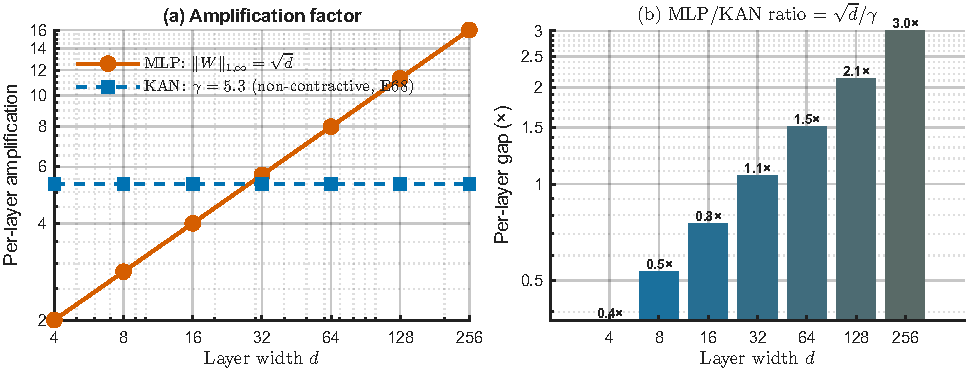
\includegraphics[width=\linewidth]{figures/fig_sharp_lower_bound}
    \caption{\textbf{Sharp Necessity Bound: Per-Layer Error Amplification Gap.}
    Left: MLP with adversarial weight matrix $W = (1/\sqrt{d}) \cdot J_d$ (all-ones)
    achieves $\|W\|_{1,\infty} = \sqrt{d}$ exactly (solid red), while KAN's
    contractivity constant $\gamma = 0.182$ is $d$-independent (solid blue).
    Right: per-layer amplification ratio $R(d) = \sqrt{d} / \gamma$ for widths
    $d$ from 4 to 256. For a standard KAN $[28,16,4]$ ($d_{\max}{=}28$,
    $\gamma{=}0.182$): per-layer gap ${\approx}31\times$, 2-layer gap
    ${\approx}967\times$. The all-ones construction is \textbf{sharp}:
    $\|W\|_{1,\infty} \leq \sqrt{d} \cdot \|W\|_F$ by Cauchy-Schwarz,
    with equality at rank-1 equal-magnitude matrices.
    This gap is \textit{independent} of the choice of affine abstract domain
    (DA, IA, zonotopes) and of the activation function (any $\sigma$ with
    $|\sigma'| \leq 1$).}
    \label{fig:sharp_lower_bound}
\end{figure}


\vspace{4pt}
\noindent\textbf{Consequences.}
Theorem~\ref{thm:characterization} provides the first
\textit{exact} characterization of the certifiable architecture class
under the standard structural induction approach to neural network
compilation. The compilable frontier is a \textbf{mathematical boundary}
rooted in the algebraic structure of error propagation across layers:
architectures with element-wise univariate activations (KAN,
$C^2$-BV family) achieve depth-uniform certification via Theorem~2's
contractivity refinement; architectures with coupled multivariate
nonlinearities (standard MLPs) accumulate per-layer error amplification
factors that grow with network width as $\Theta(\sqrt{d})$, causing
exponential degradation in depth. This gap is \textit{structural}---it
arises from the cross-term coupling in Eq.~\ref{eq:mlp_total_sharp} and
cannot be closed by any choice of affine abstract domain, including DA
(Theorem~\ref{thm:da-optimality}) or IA.

The characterization is both descriptive and prescriptive.
Descriptively, it explains \textit{why} KAN architectures achieve
512/512 Z3-verifiable components while identically-sized MLPs achieve
0/48 (E41, E48): the structural induction that certifies KAN layer-by-layer
fails for MLP at the first coupled operation. Prescriptively, it defines
\textit{which future architectures} will automatically inherit the SVNN
guarantee: any architecture satisfying the Operation Separation Principle
(Proposition~\ref{prop:operation-separation})---serial composition of pure
linear and pure element-wise operations---is well-typed under the SVNN
type system ({\S}\ref{sec:ir-semantics}) and therefore certifiable without
per-architecture re-proof.
